\documentclass[10pt]{article}
\usepackage[margin=.78in]{geometry}
\usepackage{amsmath,amssymb,booktabs,microtype,enumitem,hyperref,graphicx,float,array,tabularx}
\usepackage[T1]{fontenc}\usepackage{lmodern}
\setlist{nosep,leftmargin=*}
\hypersetup{colorlinks=true,linkcolor=blue,urlcolor=blue,hypertexnames=false}
\title{Minimal Iterative Harnesses for Learned Reasoning:\\When a Tiny Transformer Becomes a Procedure Executor}
\author{Paper 0.9 --- Model + Harness Computational Boundary}
\date{Matched Paper 0.85 protocol --- August 2026}
\begin{document}\maketitle
\begin{abstract}
Fixed Transformers have bounded forward computational depth, while many symbolic tasks have instance-dependent execution depth. We study the smallest external harness that turns a tiny Transformer from a predictor into an iterative controller, but require a five-machine comparison before attributing gains to tools: one-token output (M0), free autoregression (M1), structured scratchpad (M2), local proto-tool (M3), and explicit iterative harness (M4). The primary instrument exactly reuses Paper 0.85's shared-vocabulary, held-out-pair implication chains. Its local R0 gate passes three seeds, yet the model-only frontier is three for one-token, free-trace, and fully supervised structured generation. Completed learned M3/M4 controllers at L2/W64/H4 also have final-answer frontier three and zero acquisition probability at unseen $K=4$. Exact nested continuations to 2,000 and 4,000 updates do not move this boundary: M4 remains exactly zero at every tested $K\ge4$ for all seeds, while M3 stays near chance. Neither depth/width allocation, width/head controls, nor matched-draw diversity up to 96k examples rescues $K=4$; low-capacity controls sometimes lose training-range acquisition. Thus the local tool and explicit loop have not expanded the measured frontier under budget, architecture, or accessible-diversity scaling. Oracle T1/T2/T3 executions remain infrastructure controls, not learned evidence; the final staged intervention changes the training-depth boundary.
\end{abstract}

\section{Core idea}
A fixed Transformer computes \(y=F_\theta(x)\). The minimal harness permits
\[
s_{t+1}=F_\theta(x,s_t),
\]
where output may contain a special action token:
\[
\langle CALL,\ op,\ args\rangle.
\]
The harness deterministically evaluates the primitive, appends its typed result, and invokes the same model again.

The effective machine transition must be reported explicitly. M0 performs one final-token prediction. M1 emits an unconstrained proposition trace. M2 emits typed \texttt{STATE/DERIVE/ANSWER} tokens but receives no semantic callback. M3 may issue one local tool call; M4 repeatedly selects calls or an answer under an explicit step budget. A comparison that skips M1/M2 cannot distinguish external semantic execution from writable-state or supervision effects.

\section{Matched propositional prerequisite and dataset}
The primary experiment reuses Paper 0.85's corrected R0-v2 and recurrence Stage1-v2. Its 64-symbol vocabulary is shared across train and test and every symbol has positive input/output training coverage. Ordered implication pairs, rather than lexical items, are disjoint: 3,226 train pairs and 806 held-out pairs with zero observed leakage. The three L2/W64/H4 R0 seeds pass entailed, consequent-swap, fact-mismatch, and rule-LHS controls at 98.8--100\%. An earlier all-new-symbol condition is only a lexical/OOV-output stress and is not the local-rule prerequisite.

Proof training is bounded to $K\le3$. The matched initial test uses $K\in\{1,2,3,4,6,8\}$ with held-out edges and a query instruction that does not contain the target. An earlier query-target pilot is quarantined as invalid. Future shuffled-rule, distractor, branching, and ICL cells must preserve this generator rather than substitute an easier logic task.

\section{Required machine ladder and current evidence}
For matched architecture and task cells define
\[
K_{1\rm tok},\ K_{\rm AR},\ K_{\rm scratch},\ K_{\rm tool},\ K_{\rm harness}.
\]
Table~\ref{tab:status} distinguishes observed learned-model evidence from semantic infrastructure controls.

\begin{table}[H]\centering\small
\begin{tabular}{llll}
\toprule
Machine & Current condition & Measured frontier & Status\\\midrule
M0 & O0 final-only & 3 & observed learned model\\
M1 & O1 free trace & 3 & observed learned model\\
M2 & O2 structure, no state labels & none & observed learned model\\
M2 & O3 full derivation labels & 3 & observed learned model\\
M3 & one selected local T1 call & 3 & observed learned model\\
M4 & iterative T1 controller+harness & 3 & observed learned model\\
\bottomrule
\end{tabular}
\caption{Evidence status for the matched ladder. M3/M4 use three learned seeds; oracle-controller validation is reported separately.}\label{tab:status}
\end{table}

M0, M1, and fully supervised M2 are perfect at $K=1,2,3$ for every seed, then fail the three-seed gate at $K=4$; the $K=4$ acquisition fraction is zero for every condition. Hence
\[
K_{1\rm tok}=K_{\rm AR}=K_{\rm scratch,O3}=3,
\qquad G_{\rm recurrence}=0.
\]
O1 transition accuracy falls to 23--32\% at $K=4$ and approximately 10--20\% at $K=6,8$, with degraded termination. O2 often learns formatting/termination but no exact trajectories. This supplies a sharp model-only boundary against which the learned M3/M4 results below are compared.

\begin{figure}[H]\centering
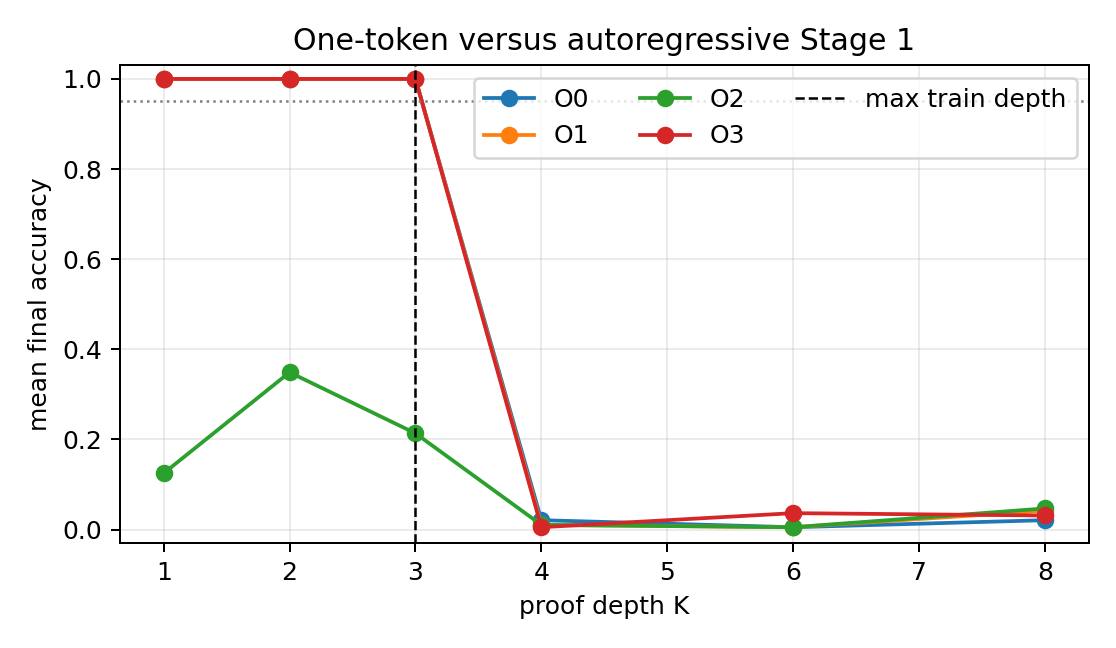
\includegraphics[width=.68\linewidth]{../paper0_85/results/recurrence_stage1_v2/figures/one_token_vs_multitoken_depth.png}
\caption{Observed Paper 0.85 model-only baselines reused unchanged. The learned M3/M4 comparison uses the same split, architecture, seeds, and depth axis.}
\end{figure}

\section{Minimal proto-tool interface}
Use the smallest action grammar:
\[
\langle CALL,\ op,\ arg_1,\ldots,arg_n\rangle
\]
and terminal
\[
\langle ANSWER,\ y\rangle.
\]
No planner, search algorithm, hidden chain-of-thought, retrieval system, or extra LLM is allowed in the primary tiny-model experiment.

Tool strength is a controlled resource. T1 evaluates only a controller-selected pair, \(\operatorname{apply}(current,rule)\to next\), and performs no search. T2 returns rules applicable to the current state, changing the selection/search burden. T3 returns the certified next proof state and is an upper control that moves most reasoning into the tool. The central condition begins with T1; T2 is introduced only to diagnose search, and T3 can never support the central model claim.

\section{CPU-validated harness semantics}
The corrected comparison infrastructure generates 384 Stage1-v2 test chains (64 at each of six depths). An explicitly oracle selecting controller executes each under T1, T2, and T3, producing 1,152 exact reference runs. All terminate correctly; calls equal $K$ and model-invocation placeholders equal $K+1$ by construction. These facts validate typed transitions, termination, and cost logging only. They do not estimate learned rule selection, call arguments, result integration, or stopping.

These oracle rows are quarantined from the learned comparison. They establish that a correct policy can use each API and that cost fields have the intended meaning, but do not fill any learned M3/M4 cell.

\section{Learned T1 controllers}
The first learned comparison fixes L2/W64/H4, 1,000 updates, seeds 11/23/37, training depths $K\le3$, and the six held-out-pair test depths. M3 receives exactly one opportunity to select a local edge; the deterministic T1 primitive returns the selected next proposition or an invalid token, after which the model emits a final answer. M4 repeatedly emits either the next proposition for T1 or \textsc{answer}; the harness performs no search. Every condition has 64 examples per depth and seed, for 2,304 preserved prediction rows.

\subsection{Metric correction}
The original M3 export named
\[
\frac{\mathbf 1\{\text{selected edge valid}\}}{K}
\]
``transition accuracy.'' This is not an accuracy over attempted transitions because M3 attempts only one call. We retain the predictions and relabel the quantity \emph{one-call edge coverage}. M3 is reported with selected-edge validity, one-call coverage, post-tool final-answer accuracy, and invalid-call rate. M4 genuinely attempts a trajectory and retains per-transition accuracy, exact-trajectory/final accuracy, termination precision and recall, invalid calls, and nontermination. M3 has no learned recurrent stopping decision, so assigning it a termination score would also be misleading.

\begin{table}[H]\centering\small
\begin{tabular}{crrrrrr}
\toprule
Machine & $K$ & Final & Execution metric & Worst seed final & $P_{\rm acquire}$ & Gate\\\midrule
M3 & 1 & 1.000 & 1.000 & 1.000 & 1.00 & pass\\
M3 & 2 & 1.000 & .500 & 1.000 & 1.00 & pass\\
M3 & 3 & 1.000 & .333 & 1.000 & 1.00 & pass\\
M3 & 4 & .021 & .076 & .000 & .00 & fail\\
M3 & 6 & .005 & .045 & .000 & .00 & fail\\
M3 & 8 & .016 & .049 & .000 & .00 & fail\\
M4 & 1 & 1.000 & 1.000 & 1.000 & 1.00 & pass\\
M4 & 2 & .995 & .997 & .984 & 1.00 & pass\\
M4 & 3 & 1.000 & 1.000 & 1.000 & 1.00 & pass\\
M4 & 4 & .000 & .000 & .000 & .00 & fail\\
M4 & 6 & .000 & .012 & .000 & .00 & fail\\
M4 & 8 & .000 & .054 & .000 & .00 & fail\\
\bottomrule
\end{tabular}
\caption{Completed learned T1 results. M3's execution metric is one-call edge coverage; M4's is per-transition accuracy. Acquisition requires final accuracy and the machine-specific execution gate to reach .95 in a seed.}
\label{tab:learned-controller}
\end{table}

\begin{figure}[H]\centering
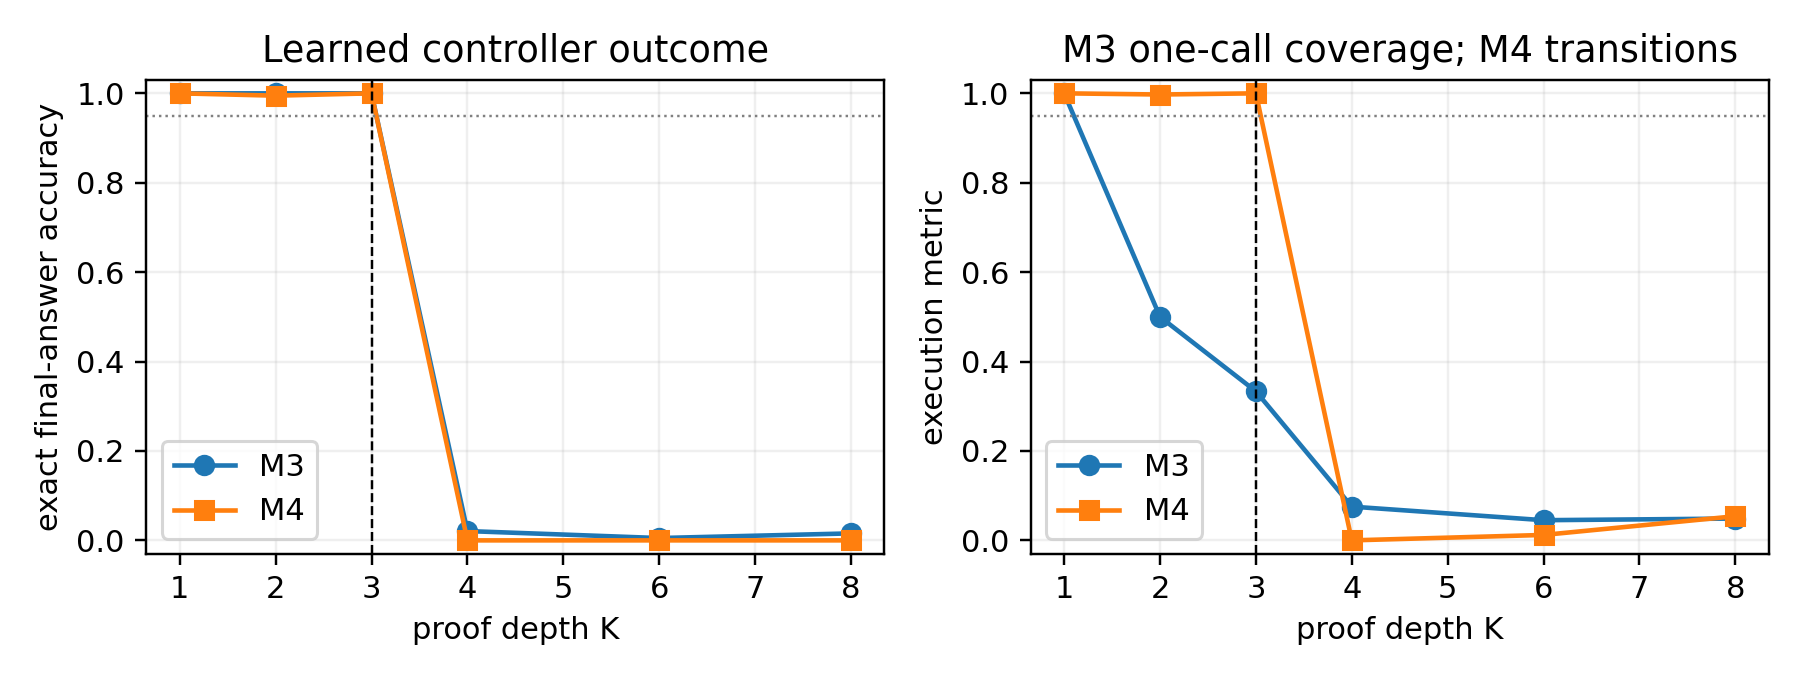
\includegraphics[width=.84\linewidth]{results/learned_controller_v1/analysis_v2/figures/learned_m3_m4_depth.png}
\caption{Learned T1 controllers. The dashed vertical line is the training boundary. M3's declining coverage inside the passing range is structural---one call covers $1/K$ of a valid chain---while M4's curve measures all required transitions.}
\label{fig:learned-controller}
\end{figure}

Both machines therefore have the contiguous frontier
\[
K_{\rm tool}=K_{\rm harness}=3,
\qquad G_{\rm tool}=G_{\rm harness}=0
\]
relative to the matched M0 frontier. M3 selects a valid first edge on every training-range evaluation. Its perfect $K=2,3$ answers cannot be attributed to tool execution of the complete proof: the one call covers only one half or one third of the chain, and the model predicts the remainder. At unseen depths, selected-edge validity itself becomes unstable (mean .302, .271, and .391 at $K=4,6,8$), while exact answers fall below 2.1\%.

M4 provides the stronger semantic machine but does not acquire a longer procedure. It is exact at $K=1,3$ and reaches 99.5\% mean final accuracy at $K=2$ (worst seed 98.4\%). At every tested $K\ge4$, exact final and trajectory accuracy are zero. Invalid-action rates are 100\% at $K=4,6$ and 98.96\% at $K=8$ when pooled across seeds; no example is classified as a max-step nontermination. Correct termination recall is zero beyond the training boundary because invalid actions usually end the trajectory before a valid stop. This is a train-short/test-long acquisition failure, not evidence that T1 or an ideal iterative controller lacks the representational ability to traverse longer chains.

\section{Later extension: tree primitives}
Begin with one primitive:
\[
parent(x)\rightarrow y
\]
plus a root/no-parent signal. Add children, equality, or level primitives only if necessary.

\section{Later relational tasks}
Compare model-only with model+harness on:
\[
parent(x),\ grandparent(x),\ root(x),\ isAncestor(x,y),
\]
\[
sameParent(x,y),\ sameGrandparent(x,y),\ sameAncestorAtLevel_k(x,y).
\]
Vary tree depth, branching, distractors, and required traversal independently.
These experiments follow the propositional M0--M4 comparison. Existing deterministic tree reference controllers validate the harness API but are not learned-model evidence.

\section{Closure hypothesis}
For a fixed model, \(d_{\max}<\infty\) may persist even with scale. For a harnessed model, if local transition competence is reliable,
\[
T_{\rm steps}\approx O(d)
\]
should permit much larger relation depth. The key question is whether the learned controller generalizes:
\[
\text{call parent; update state; test stop; repeat}.
\]

\section{Cross-paper benchmark families}
Paper 0.5 supplies bounded pattern/refinement tasks; Paper 0.6 supplies semantic/tree relations; Paper 0.7 supplies propositional proof chains and first-order unification; Paper 0.8 supplies copy, contextual task selection, and structured rule induction. Not every task requires a tool: the objective is to determine where iteration changes the competence class.

\section{Tiny-model phase diagram and staged next experiment}
Vary model resources \(L,W,H\) and harness budget \(T_{\max}\). Compare:
model-only, one callback, bounded loop, and loop until a learned stop condition.

The completed three-seed result licenses a bounded resource diagnostic, not the old 1,620-cell factorial. The v3 staged plan first tests exact 2$\times$/4$\times$ continuation of L2/W64/H4, then depth and parameter-matched deep/narrow versus shallow/wide allocation. Width/head controls are conditional; training-example diversity at fixed $K_{\max}=3$ and a separate $K_{\max}=3$ versus 4 boundary test follow only for the selected architecture. Each stage stops on rescue or futility gates.

Stage A replays from step zero under the v3 exact checkpoint contract and takes nested snapshots at 2,000 and 4,000 updates. Checkpoints preserve model and optimizer state, Python/NumPy/Torch/MPS RNG state, the data-stream cursor, and configuration/dataset hashes; an interrupted-versus-uninterrupted CPU test produces bitwise-identical weights and identical metric rows.

\begin{table}[H]\centering\small
\begin{tabular}{crrrr}
\toprule
Machine & Updates & $K\le3$ final & $K=4$ mean/worst & Final frontier\\\midrule
M3 & 2,000 & 1.000 & .016/.000 & 3\\
M3 & 4,000 & 1.000 & .010/.000 & 3\\
M4 & 2,000 & 1.000 & .000/.000 & 3\\
M4 & 4,000 & 1.000 & .000/.000 & 3\\
\bottomrule
\end{tabular}
\caption{Completed three-seed Stage-A budget continuation. The frontier shown is final-answer competence. Under the stricter machine-specific execution gate, M3's one-call coverage is structurally below .95 for $K>1$, while M4's frontier remains three.}
\label{tab:stage-a}
\end{table}

More optimization preserves acquisition on the training support but does not produce procedure-length extrapolation. M3's mean final accuracy at $K=4$ changes from .016 at 2,000 updates to .010 at 4,000; M4 is zero at $K=4,6,8$ under both snapshots for every seed. Stage A satisfies the preregistered completion prerequisite for Stage B, but not a rescue claim.

Stage B compares a four-layer width-64 model (147,072 parameters), a four-layer width-48 parameter-matched model (85,728), and a one-layer width-88 parameter-matched model (81,048). None acquires $K=4$: M4 is exactly zero at $K=4,6,8$ in all 54 seed--depth extrapolation cells. Both four-layer models retain M4 frontier three. The shallow matched model also has M4 frontier three, although its training-range means fall slightly to .995 and .984 at $K=2,3$. Its M3 arm fails acquisition even within the training range (means .458, .557, .505), whereas both deeper M3 arms remain perfect through $K=3$ and near zero beyond it. Under the preregistered execution metric, their M3 frontier is one because a single call covers only $1/K$ of a multi-edge proof.

The allocation comparison therefore supplies no procedure-length rescue and no unique shared winner: M4 ties at three across all allocations, while the M3 winner set ties the two deeper models. This unresolved allocation result activates Stage C's width/head controls; it does not license a claim that depth is irrelevant outside the measured cells.

Stage C varies width and head count at two layers. Narrow, wide, and eight-head models reproduce the strict M3/M4 frontiers 1/3; none acquires $K=4$. The one-head model has frontier zero for both machines, showing an acquisition failure rather than a useful extrapolation tradeoff. Width and additional head allocation therefore do not resolve the Stage-B tie or move the procedure-length boundary. Because no resource arm improves the first failed depth in every seed, the architecture branch is futile under the encoded rescue rule. The matched-draw diversity intervention proceeds with the deterministic selected architecture; its result must be interpreted as a data-support test, not further architecture search.

Stage D selects the narrow model deterministically after the tied architecture frontiers and exposes it to exact-prefix pools of 24k, 48k, or 96k distinct examples while holding 96k ordered draws fixed. No pool produces any $K=4$ acquisition: M4 final accuracy is zero for every seed at $K=4,6,8$, and M3 remains at or below .026 mean. More diversity also does not monotonically improve acquisition. The M4 strict frontier is two for 24k and 96k but only one for 48k because some training-range seed gates fall below .95; M3 remains at one throughout. This is a negative accessible-diversity result for the selected low-capacity architecture, not evidence that diversity is generally irrelevant. The preregistered selector chooses 24k by max-min frontier, summed frontier, then minimum pool size for Stage E.

\section{Minimality}
Shrink model size, special-token grammar, tool primitives, state fields, and maximum steps. The target is the smallest model+harness pair that exhibits systematic depth extrapolation unavailable to the model alone.

\section{Reproducibility and evidence boundary}
Matched generator construction is in \path{recurrence_chains.py}. Typed T1/T2/T3 semantics are in \path{proof_harness.py}; the comparison and status runners use the \path{paper09_paper085_*} prefix. Configuration \path{paper085_comparison_v2.json} pins the corrected shared-vocabulary split. Artifacts under \path{results/paper085_comparison_v2} contain the oracle-controller validation and explicitly record \texttt{learned\_model\_results=false}.

Learned checkpoints and immutable legacy exports are under \path{results/learned_controller_v1}. The semantic-v2 analysis preserves all 2,304 predictions, pins the source SHA-256, and writes corrected raw rows, seed/depth summaries, three-seed frontiers, a manifest, and Figure~\ref{fig:learned-controller} under \path{analysis_v2}. Configurations \path{learned_controller_v3_staged.json} and \path{learned_controller_v3_cells.csv}, with the companion plan manifest, preregister the bounded stages. Stage runners use the corresponding \path{paper09_learned_controller_stage_*} modules. Tracked A/B/C/D artifact directories contain 4,608, 6,912, 9,216, and 6,912 prediction rows, per-seed/depth summaries, losses, complete frontier tables, and hash-linked manifests. Checkpoint tensors are excluded from version control.

\section{Appendix: pretrained models}
Use small pretrained models only as external validation, separating direct answer, proto-tool harness, native tool calling, and native reasoning/scratchpad modes where available. Corpus exposure and learned procedures remain uncontrolled.

\section{Conclusion}
Paper 0.9 asks where systematicity comes from when the same learned local operator is embedded in a minimal iterative machine. Local implication is reliably acquired, but one-token, free-trace, fully supervised structured, one-call T1, and iterative T1 machines all stop at measured depth three in the initial matched regime. Exact continuation through four times the original optimization budget, depth/width and head controls, and matched-draw diversity through 96k examples leave $K=4$ unacquired; low-capacity conditions can instead lose training-range competence. The learned M4 harness changes the available computation but does not yield a train-short/test-long controller in these cells. These are finite negative acquisition results, not impossibility or closure claims. The remaining preregistered intervention asks whether adding $K=4$ training examples changes the boundary.
\end{document}
